\documentclass[12pt,a4paper]{article}
\usepackage[utf8]{inputenc}
\usepackage[T1]{fontenc}
\usepackage{geometry}
\usepackage{graphicx}
\usepackage{hyperref}
\usepackage{xcolor}
\usepackage{titlesec}
\usepackage{fancyhdr}
\usepackage{tabularx}
\usepackage{colortbl}
\usepackage{booktabs}
\usepackage{enumitem}
\usepackage{pgfplots}
\pgfplotsset{compat=1.18}
\usepackage{tikz}
\usetikzlibrary{shapes.geometric, arrows.meta, positioning}
\usepackage{multirow}
\usepackage{float}

% Page setup
\geometry{a4paper, margin=1in}

% Colors
\definecolor{primary}{RGB}{0, 102, 204}
\definecolor{lightgray}{RGB}{240, 240, 240}

% Header/footer
\pagestyle{fancy}
\fancyhf{}
\fancyhead[L]{\small\textcolor{gray}{Report Title}}
\fancyhead[R]{\small\textcolor{gray}{\today}}
\fancyfoot[C]{\small\thepage}
\renewcommand{\headrulewidth}{0.4pt}

% Section styling
\titleformat{\section}
    {\Large\bfseries\color{primary}}{\thesection}{0.5em}{}
\titleformat{\subsection}
    {\large\bfseries}{}{0em}{}

% Hyperlinks
\hypersetup{colorlinks=true, linkcolor=primary, urlcolor=primary}

\title{\textbf{Report Title} \\ \large Subtitle or Description}
\author{Author Name \\ Organization}
\date{\today}

\begin{document}

\maketitle
\thispagestyle{empty}
\newpage

\tableofcontents
\newpage

% --- EXECUTIVE SUMMARY ---
\section{Executive Summary}
Brief overview of the report's key findings and recommendations.

% --- INTRODUCTION ---
\section{Introduction}
Context and background for the report.

% --- DATA / FINDINGS ---
\section{Findings}

\subsection{Key Metrics}

\begin{table}[htbp]
\centering
\begin{tabularx}{0.9\textwidth}{lXrr}
\toprule
\textbf{Metric} & \textbf{Description} & \textbf{Value} & \textbf{Change} \\
\midrule
Metric 1 & Description of metric & 1,234 & +12\% \\
Metric 2 & Description of metric & 5,678 & -3\% \\
Metric 3 & Description of metric & 910 & +25\% \\
\bottomrule
\end{tabularx}
\caption{Summary of key metrics}
\end{table}

\subsection{Analysis}
Detailed analysis of findings with supporting data.

% --- EXAMPLE: Bar Chart ---
\begin{figure}[H]
\centering
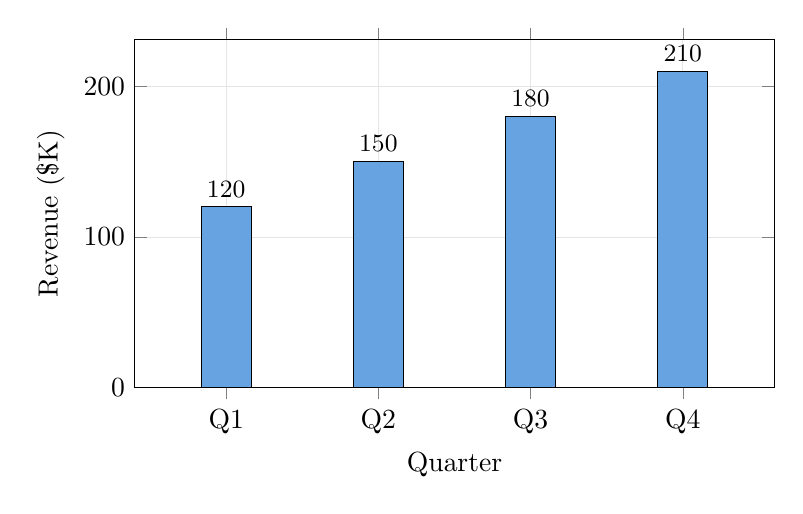
\begin{tikzpicture}
\begin{axis}[
    ybar,
    width=0.8\textwidth,
    height=6cm,
    xlabel={Quarter},
    ylabel={Revenue (\$K)},
    symbolic x coords={Q1, Q2, Q3, Q4},
    xtick=data,
    nodes near coords,
    nodes near coords style={font=\small\bfseries},
    bar width=18pt,
    ymin=0,
    grid=major,
    major grid style={thin, gray!20},
    enlarge x limits=0.2,
]
\addplot[fill=primary!60] coordinates {(Q1,120) (Q2,150) (Q3,180) (Q4,210)};
\end{axis}
\end{tikzpicture}
\caption{Quarterly revenue performance}
\label{fig:revenue}
\end{figure}

% --- EXAMPLE: Process Flowchart ---
\subsection{Process Overview}

\begin{figure}[H]
\centering
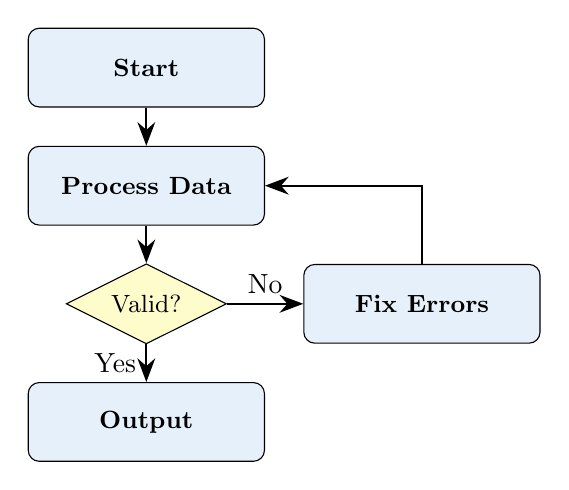
\begin{tikzpicture}[
    node distance=1.5cm,
    box/.style={draw, rounded corners, fill=primary!10, minimum width=3cm, minimum height=1cm, align=center, font=\small\bfseries},
    decision/.style={draw, diamond, fill=yellow!20, minimum width=1.5cm, aspect=2, align=center, font=\small},
    arrow/.style={-{Stealth[length=3mm]}, thick}
]
\node[box] (start) {Start};
\node[box, below of=start] (process) {Process Data};
\node[decision, below of=process] (check) {Valid?};
\node[box, below of=check] (output) {Output};
\node[box, right of=check, node distance=3.5cm] (fix) {Fix Errors};

\draw[arrow] (start) -- (process);
\draw[arrow] (process) -- (check);
\draw[arrow] (check) -- node[left] {Yes} (output);
\draw[arrow] (check) -- node[above] {No} (fix);
\draw[arrow] (fix) |- (process);
\end{tikzpicture}
\caption{Data processing workflow}
\label{fig:workflow}
\end{figure}

% --- RECOMMENDATIONS ---
\section{Recommendations}
\begin{enumerate}[itemsep=0.5em]
    \item First recommendation with rationale
    \item Second recommendation with rationale
    \item Third recommendation with rationale
\end{enumerate}

% --- CONCLUSION ---
\section{Conclusion}
Summary of findings and next steps.

% --- APPENDIX (optional) ---
% \appendix
% \section{Supplementary Data}

\end{document}
